\documentclass{article}[a4paper]
\usepackage[a4paper, left=2.5cm,right=2cm,top=2.5cm,bottom=2.5cm]{geometry}
\usepackage[utf8]{inputenc}
\usepackage{csquotes}
\usepackage{booktabs}
\usepackage{amsmath}
\usepackage{mathtools}% http://ctan.org/pkg/mathtools
\usepackage{caption}
\captionsetup{width=.75\textwidth}
\usepackage[usestackEOL]{stackengine}
\usepackage{float}
\usepackage{subcaption}
\usepackage{tikz}
\usetikzlibrary{shapes.geometric,arrows,positioning,fit}
\usetikzlibrary{shapes,calc,arrows}
\usepackage{natbib}
\usepackage{graphicx}
\usepackage{subfiles}
\usepackage{blindtext}
\usepackage{hyperref}
\usepackage{float}
\usepackage{physics} % for 'pdv' macro
\usepackage{qtree}
\usepackage{stmaryrd}
\usepackage{multicol}
\usepackage{xparse}
\usepackage{amssymb}
\usepackage{xcolor}
\usepackage{neuralnetwork}
\usepackage{pgfplots}
\usepackage{sidecap}
 
\usepackage{tikz}
\usetikzlibrary{decorations.pathreplacing}

\pgfplotsset{compat=1.16}

% Syntax: \colorboxed[<color model>]{<color specification>}{<math formula>}
\newcommand*{\colorboxed}{}
\def\colorboxed#1#{%
  \colorboxedAux{#1}%
}
\newcommand*{\colorboxedAux}[3]{%
  % #1: optional argument for color model
  % #2: color specification
  % #3: formula
  \begingroup
    \colorlet{cb@saved}{.}%
    \color#1{#2}%
    \boxed{%
      \color{cb@saved}%
      #3%
    }%
  \endgroup
}

\def\XXX#1{\textcolor{red}{XXX #1}}

\NewDocumentCommand{\codeword}{v}{%
\texttt{\textcolor{blue}{#1}}%
}
\newcommand\Mycomb[2][^n]{\prescript{#1\mkern-0.5mu}{}C_{#2}}
\def\XXX#1{\textcolor{red}{XXX #1}}
\newcommand{\vect}[1]{\boldsymbol{\textcolor{blue}{#1}}}

\title{\textbf{Elements of Machine Learning}\\
Assigment 1 - Problem 4
}
\author{ Sangeet Sagar(7009050), Philipp Schuhmacher(7010127)\\
        \texttt{\{sasa00001,phsc00003\}@stud.uni-saarland.de}
}
% \pgfplotsset{compat=1.17}
% \parindent 0in
% \parskip 0em
\begin{document}
\maketitle
\section*{Curse of dimensionality}
\subsection*{Part 1}
\textcolor{red}{Explain when the so-called \textit{curse of dimensionality} occurs. Describe the phenomenon in your own words.}\\
Often with lot of input features, the feature space becomes high-dimensional. That is to say, number of required samples increases exponentially with the number of dimensions. The curse of dimensionality states that if our number of dimension gets bigger, we need more data to generalize.

\subsection*{Part 2}
\textcolor{red}{Exercise 4.7.4 in ISLR. Please answer the following questions with regard to observations $x \in X$ taking values in the interval [0.05, 0.95].}\\

\subsubsection*{a}
\textcolor{red}{Suppose that we have a set of observations, each with measurements on $p = 1$ feature, $X$. We assume that $X$ is uniformly distributed in $[0,1]$. Associated with each observation is a response value. Suppose that we wish to predict a test observation’s response using only observations that are within $10\%$ of the range of $X$ closest to that test observation. For instance, in order to predict the response for a test observation with $X=0.6$, we will use observations in the range $[0.55, 0.65]$. On average, what fraction of the available observations will we use to make the prediction?}\\

\begin{figure}[H]
    \centering
    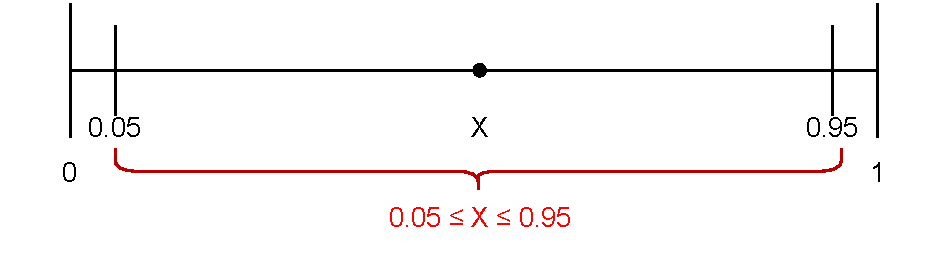
\includegraphics[width=4in]{HW1/hw1_q4_1.pdf}
\end{figure}

\begin{figure}[H]
    \centering
    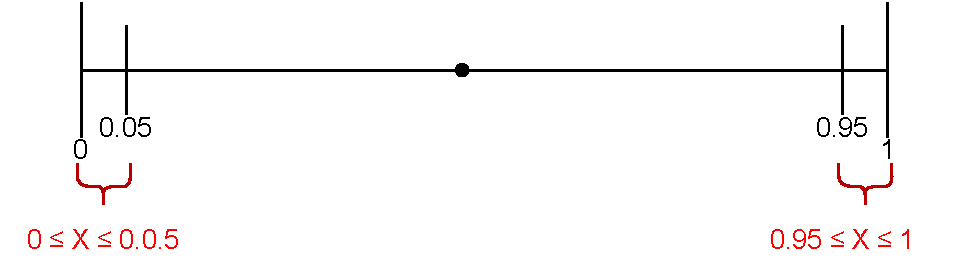
\includegraphics[width=4in]{HW1/hw1_q4_2.pdf}
\end{figure}
\begin{enumerate}
    \item The first figure illustrates the interval when $X \in [0.05, 0.95]$. Therefore, for each associated response corresponding to $X$ to lie within $10\%$ of the range of $X$ is given by $[X-0.05, X+0.05]$ i.e. 0.05 units on the either side of $X$ as to cover a length of 0.1 which is $10\%$ of the range of $X$
    \item The second picture illustrates when $X \in [0, 0.05)$. Therefore, for each associated response corresponding to $X$, it would lie in the interval $[0, X+0.05]$. Here we have lower bound as $0$, because there is no room to cover the range to the left of $X$. For e.g. if $X=0.02$, it can only cover range on its right i.e. $0.02+0.05$, while to the left $0.02-0.05$ is out of the given interval.
    \item Similarly for $X \in (0.95, 1]$, the interval used to predict the responses would be $[X-0.05, 1]$. Because it can only take the range of 0.05 units towards its left.
\end{enumerate}
 Now in order to average fraction of available observation, we use 
 \begin{align*}
     f_{ave} = \frac{1}{b-a} \int_{a}^{b} f(x) dx
 \end{align*}
where $f(x)$ in our case would be the length of the interval.
\begin{enumerate}
    \item For interval: $[0.05 \leq X \leq 0.95]$:  Observation interval: $[X-0.05, X+0.05]$.\\ Length of the interval = $0.1$
    \item For interval: $[0 \leq X < 0.05]$: Observation interval: $[0, X+0.05]$.\\ Length of the interval = $X+0.05 - 0 = X+0.05$
    \item For interval: $[0.95 < X \leq 1]$: Observation interval: $[X-0.05, 1]$.\\ Length of the interval = $1 - (X-0.05) = 1.05-X$
\end{enumerate}
We have
\begin{align*}
    f_{ave} &= \frac{1}{(1-0)} \left[ \int_{0}^{0.05} (x+0.05) dx + \frac{1}{(0.95-0.05)} \int_{0.05}^{0.95} (0.1) dx + \frac{1}{(1-0.95)} \int_{0.95}^{1} (1.05-x) dx \right]\\
    &= (0.00125+0.0025) + (0.09) + (0.0525-0.04875)\\
    &= 0.0975
\end{align*}
Therefore, it can be concluded that on an average $9.75\%$ of available observations we will be using to make predictions.

\subsubsection*{b}
\textcolor{red}{Now suppose that we have a set of observations, each with measurements on $p=2$ features, $X_1$ and $X_2$ . We assume that $(X_1 , X_2)$ are uniformly distributed on $[0,1]\times[0,1]$. We wish to predict a test\\ observation’s response using only observations that are within $10\%$ of the range of $X_1$ and $X_2$ closest to that test observation. On average, what fraction of the available observations will we use to make the prediction?}\\
On a similar note, for $X_1$ we know that on an average $9.75\%$ of the available observation will be used. Similarly, for $X_2$ we will have $9.75\%$. Hence, for $(X_1, X_2)$ being uniformly distributed, we will have $0.0975 \times 0.0975 = 9.5e-3$ as the average fraction or $0.95\%$  of available observation used to make prediction

\subsubsection*{c}
\textcolor{red}{Now suppose we have a set of observations on $p=m$ features. In the same scenario as before, we wish to predict a test observation’s response using only observations that are within $10\%$ of each feature’s range that is closest to that test observation. On average, what fraction of the available observations will we use to make the prediction?}\\
Following from the last part, we will have $0.0975^m$ as the average fraction of the available observations to make predictions.

\subsubsection*{d}
\textcolor{red}{Now suppose that we wish to make a prediction for a test observation by creating a p-dimensional hypercube centered around the test observation that contains, on average, $10\%$ of the training observations. For p=1,2, and 100, what is the length of each side of the hypercube? Comment on your answer. Note: A hypercube is a generalization of a cube to an arbitrary number of dimensions. When $p=1$, a hypercube is simply a line segment, when $p=2$ it is a square, and when $p=100$ it is a 100-dimensional cube.}\\
Given that each p-dimensional hypercube would contain $10\%$ of the training observations or 0.1 as the fraction of training observations.
\begin{enumerate}
    \item For $p=1$: the hypercube is simply a line. Hence length of the line=0.1 units.
    \item For $p=2$: the hyperbole is square for which the area associated is 0.1. Hence length side of each side of square is given as $\sqrt{0.1} = 0.31$ units.
    \item For $p=100$: the hyperbole is a 100-dimension cube. The volume associated is 0.1. Hence length of each side is given as $0.1^(\frac{1}{100}) = 0.977$.
\end{enumerate}
\bibliographystyle{plainnat}
\bibliography{references}
\end{document}